% Author: Izaak Neutelings (June 2020)
\documentclass[border=3pt,tikz]{standalone}
\usetikzlibrary{calc}
\tikzset{>=latex} % for LaTeX arrow head

% METHOD 1: \newcommand
\newcommand\rightAngle[4]{
  \pgfmathanglebetweenpoints{\pgfpointanchor{#2}{center}}{\pgfpointanchor{#1}{center}}
  \coordinate (tmpRA) at ($(#2)+(\pgfmathresult+45:#4)$);
  \draw[blue!80!black] ($(#2)!(tmpRA)!(#1)$) -- (tmpRA) -- ($(#2)!(tmpRA)!(#3)$);
  %\fill[red] (tmpRA) circle(0.02);
}

% METHOD 2: \pic
\tikzset{
  pics/rightangle/.style args={(#1)-(#2)-(#3):#4}{
    code={
      \pgfmathanglebetweenpoints{\pgfpointanchor{#2}{center}}{\pgfpointanchor{#1}{center}}
      \coordinate (tmpRA) at ($(#2)+(\pgfmathresult+45:#4)$);
      \draw[green!80!black] ($(#2)!(tmpRA)!(#1)$) -- (tmpRA) -- ($(#2)!(tmpRA)!(#3)$);
    }
  }
}

% METHOD 3: \def by Alexandros Tsagkaropolulos
\def\MarkRightAngle[size=#1](#2,#3,#4){
  \draw[red!80!black] ($(#3)!#1!(#2)$) -- ($($(#3)!#1!(#2)$)!#1!90:(#2)$) -- ($(#3)!#1!(#4)$)
}

% METHOD 4: \pic with filled area
\tikzset{
  narcs/.initial=1,      % number of (dark) arcs
  nmarks/.initial=0,     % number of marks to indicate equal angles
  marklen/.initial=0.27, % length of marks
  markdist/.initial=3,   % distance between marks
  angshift/.initial=1,   % shift from origin
  angcol/.style={draw=#1,fill=#1!40}, % shorthand to fill (light) & draw (dark)
  angcol/.default={myblue},
  pics/mark angle/.style args={(#1)-(#2)-(#3):#4}{ % arc: any angle
    code={
      \tikzset{narcs/.get=\narcs}
      \tikzset{nmarks/.get=\nmarks}
      \tikzset{marklen/.get=\marklen}
      \tikzset{markdist/.get=\markdist}
      \tikzset{angshift/.get=\angshift}
      \pgfmathanglebetweenpoints{\pgfpointanchor{#2}{center}}{\pgfpointanchor{#1}{center}}
      \pgfmathsetmacro\tmpAngA{\pgfmathresult}
      \pgfmathanglebetweenpoints{\pgfpointanchor{#2}{center}}{\pgfpointanchor{#3}{center}}
      \pgfmathsetmacro\tmpAngB{\tmpAngA<\pgfmathresult?\pgfmathresult:\pgfmathresult+360}
      \pgfmathsetmacro\tmpAveAng{(\tmpAngA+\tmpAngB)/2}
      \coordinate (tmpS) at (\tmpAveAng:{\angshift*0.006/abs(sin((\tmpAngB-\tmpAngA)/2))}); % shift
      \coordinate (tmp#2) at ($(#2)+(tmpS)$);
      \coordinate (tmpA) at ($(tmp#2)+(\tmpAngA:#4)$);
      \fill[pic actions,draw=none] % fill circle segment
        (tmp#2) -- (tmpA) arc(\tmpAngA:\tmpAngB:#4) -- cycle;
      \draw[pic actions,fill=none] (tmpA) arc(\tmpAngA:\tmpAngB:#4);
      \ifnum\narcs>0
        \foreach \i [evaluate={\dr=0.02*\markdist*(\i-1);}] in {1,...,\narcs}{
          \draw[pic actions,fill=none] % draw angle mark
          (tmpA)++(\tmpAngA:-\dr) arc(\tmpAngA:\tmpAngB:#4-\dr);
        }
      \fi
      \ifnum\nmarks>0
        \foreach \i [evaluate={\a=\tmpAveAng+\markdist/(#4)*(\i-0.5-\nmarks/2);}]
          in {1,...,\nmarks}{
          \draw (tmp#2)++(\a:{#4-\marklen*max(#4/2,\marklen)})
            --++ ({(\a+2*\tmpAveAng)/3}:{2*\marklen*max(#4/2,\marklen)});
      }
      \fi
    }
  },
  pics/right angle/.style args={(#1)-(#2)-(#3):#4}{ % right angle
    code={
      \tikzset{angshift/.get=\angshift}
      \pgfmathanglebetweenpoints{\pgfpointanchor{#2}{center}}{\pgfpointanchor{#1}{center}}
      \pgfmathsetmacro\tmpAngA{\pgfmathresult}
      %\pgfmathanglebetweenpoints{\pgfpointanchor{#2}{center}}{\pgfpointanchor{#1}{center}}
      %\pgfmathsetmacro\tmpAveAng{(\tmpAngA+(\tmpAngA>\pgfmathresult?\pgfmathresult:\pgfmathresult+360))/2}
      \coordinate (tmpS) at (\tmpAngA+45:\angshift*0.008); % shift
      \coordinate (tmp#1) at ($(#1)+(tmpS)$);
      \coordinate (tmp#2) at ($(#2)+(tmpS)$);
      \coordinate (tmp#3) at ($(#3)+(tmpS)$);
      \coordinate (tmpRA) at ($(tmp#2)+(\tmpAngA+45:#4)$);
      \fill[pic actions,draw=none] % fill square area
        ($(tmp#2)!(tmpRA)!(tmp#1)$) -- (tmpRA) -- ($(tmp#2)!(tmpRA)!(tmp#3)$) -- (tmp#2) -- cycle;
      \draw[pic actions,fill=none] % draw orthogonal mark
        ($(tmp#2)!(tmpRA)!(tmp#1)$) -- (tmpRA) -- ($(tmp#2)!(tmpRA)!(tmp#3)$);
    }
  }
}

\begin{document}


% RIGHT ANGLE: METHOD 1 with \newcommand
\foreach \ang in {0,20}{ %,90,120,180}{
  \begin{tikzpicture}
    \coordinate (O) at (0,0);
    \coordinate (X) at (\ang:1);
    \coordinate (Y) at (\ang+90:1);
    \draw (X) -- (O) -- (Y);
    \rightAngle{X}{O}{Y}{0.40}
  \end{tikzpicture}
}


% RIGHT ANGLE: METHOD 2 with \pic
\foreach \ang in {0,20}{%,120,220,340
  \begin{tikzpicture}
    \coordinate (O) at (0,0);
    \coordinate (X) at (\ang:1);
    \coordinate (Y) at (\ang+90:1);
    \draw (X) -- (O) -- (Y);
    \pic {rightangle={(X)-(O)-(Y):0.4}};
    \node[scale=0.7] at (45+\ang:0.8) {pic};
  \end{tikzpicture}
}


% RIGHT ANGLE: METHOD 3 with \def
\foreach \ang in {0,20}{%,120,220,340
  \begin{tikzpicture}
    \coordinate (O) at (0,0);
    \coordinate (X) at (\ang:1);
    \coordinate (Y) at (\ang+90:1);
    \draw (X) -- (O) -- (Y);
    \MarkRightAngle[size=8 pt](X,O,Y);
    \node[scale=0.7] at (45+\ang:0.8) {def};
  \end{tikzpicture}
}


% RIGHT ANGLE METHOD 4: \pic with fill
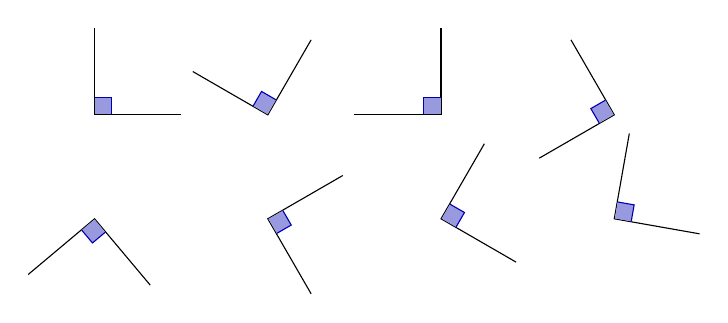
\begin{tikzpicture}[scale=1.1]
  \foreach \ang [count=\i from 0,evaluate={\x=2*mod(\i,4); \y=-1.2*floor(\i/4);}]
                 in {0,60,90,120,220,300,330,350}{
    \begin{scope}[shift={(\x,\y)}]
      \coordinate (O) at (0,0);
      \coordinate (X) at (\ang:1);
      \coordinate (Y) at (\ang+90:1);
      \draw (X) -- (O) -- (Y);
      \pic[angcol=blue!70!black] {right angle={(X)-(O)-(Y):0.3}};
      %\pic[angcol=green!70!black] {right angle={(Y)-(O)-(X):0.3}};
    \end{scope}
  }
\end{tikzpicture}


% METHOD 4: ROUND ANGLE
\foreach \nmark/\narc in {0/1,1/1,2/1,0/2,0/3}{
  \message{^^JRound angles: Number of marks \nmark}
  \begin{tikzpicture}[scale=1.1]
    \foreach \dang [count=\i from 0] in {10,40,90,130,180,220,300,350}{
      \foreach \ang [count=\j from 0,evaluate={\x=2*mod(\i,4); \y=-1.4*\j-4.2*floor(\i/4);}]
                       in {0,40,170}{ % rotate whole frame
        \begin{scope}[shift={(\x,\y)}]
          \coordinate (O) at (0,0);
          \coordinate (X) at (\ang:1);
          \coordinate (Y) at (\ang+\dang:1);
          \draw (X) -- (O) -- (Y);
          \pic[angcol=blue!70!black,nmarks=\nmark,narcs=\narc] {mark angle={(X)-(O)-(Y):0.3}};
          \pic[angcol=green!70!black,nmarks=\nmark,narcs=\narc] {mark angle={(Y)-(O)-(X):0.2}};
          %\fill[black] (O) circle(0.02);
        \end{scope}
      }
    }
  \end{tikzpicture}
}

% ORTHOGONAL PROJECTION
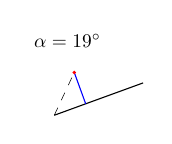
\begin{tikzpicture}[scale=1.2]
  \def\ang{20}
  \coordinate (O) at (0,0);
  \coordinate (R) at (\ang:1);
  \pgfmathanglebetweenpoints{\pgfpointanchor{O}{center}}{\pgfpointanchor{R}{center}}
  \pgfmathsetmacro\tmpAng{int(\pgfmathresult)}
  \draw (O) -- (R);
  \coordinate (RA) at ($(O)+(\pgfmathresult+45:0.5)$);
  \draw[dashed,very thin] (O) -- (RA);
  \draw[blue] ($(O)!(RA)!(R)$) -- (RA); % project
  \fill[red] (RA) circle(0.02);
  \node[scale=0.7] at (80:0.8) {$\alpha=\tmpAng^\circ$};
\end{tikzpicture}


% ORTHOGONAL PROJECTION
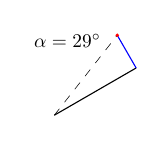
\begin{tikzpicture}[scale=1.2]
  \def\ang{30}
  \coordinate (O) at (0,0);
  \coordinate (R) at (\ang:1);
  \pgfmathanglebetweenpoints{\pgfpointanchor{O}{center}}{\pgfpointanchor{R}{center}}
  \pgfmathsetmacro\tmpAng{int(\pgfmathresult)}
  \draw (O) -- (R);
  \coordinate (RA) at ($(R)+(\pgfmathresult+90:0.4)$);
  \draw[dashed,very thin] (O) -- (RA);
  \draw[blue] ($(O)!(RA)!(R)$) -- (RA); % project
  \fill[red] (RA) circle(0.02);
  \node[scale=0.7] at (80:0.8) {$\alpha=\tmpAng^\circ$};
\end{tikzpicture}


% ORTHOGONAL PROJECTION
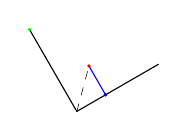
\begin{tikzpicture}[scale=1.2]
  \def\d{10pt}
  \def\ang{30}
  \coordinate (O) at (0,0);
  \coordinate (R) at (\ang:1);
  \coordinate (RT) at (\ang+90:1);
  \coordinate (RP) at ($(O)!\d!(R)$);
  \coordinate (RA) at ($(RP)!\d!90:(R)$);
  \draw (R) -- (O) -- (RT);
  \draw[dashed,very thin] (O) -- (RA);
  \draw[blue] ($(O)!(RA)!(R)$) -- (RA);
  \fill[red] (RA) circle(0.02);
  \fill[blue] (RP) circle(0.02);
  \fill[green] (RT) circle(0.02);
\end{tikzpicture}


\end{document}